\documentclass[conference]{IEEEtran}
\usepackage{amsmath,amssymb}
\usepackage{booktabs}
\usepackage{multirow}
\usepackage{graphicx}
\usepackage{xcolor}
\usepackage{tikz}
\usetikzlibrary{positioning,arrows.meta,shapes.geometric,fit}
\usepackage{pgfplots}
\pgfplotsset{compat=1.16}
\usepackage[hidelinks]{hyperref}
\usepackage{cite}

\newcommand{\sfn}{SchemaFlexTabNet-QC}
\newcommand{\htn}{HybridTabNet-QC}

\begin{document}

\title{Duplicate Contamination, Schema Loss, and Cross-Cohort Generalization in Public Cardiovascular Risk Benchmarks: A Reproducibility Audit and a Schema-Flexible Tabular Transformer}

\author{
\IEEEauthorblockN{\small 1\textsuperscript{st} Raja Rathan\\Paida}
\IEEEauthorblockA{\scriptsize\textit{Dept.\ of Artificial Intelligence}\\
\textit{SVNIT}\\
Surat, India\\
paidarajarathan@gmail.com}
\and
\IEEEauthorblockN{\small 2\textsuperscript{nd} Sanapala\\Sanjay}
\IEEEauthorblockA{\scriptsize\textit{Dept.\ of Artificial Intelligence}\\
\textit{SVNIT}\\
Surat, India\\
sanapalasanju@gmail.com}
\and
\IEEEauthorblockN{\small 3\textsuperscript{rd} Chinnapureddy\\Pavan Kumar Reddy}
\IEEEauthorblockA{\scriptsize\textit{Dept.\ of Artificial Intelligence}\\
\textit{SVNIT}\\
Surat, India\\
pavanchinnapureddy@gmail.com}
\and
\IEEEauthorblockN{\small 4\textsuperscript{th} Golla\\Abhinav Kumar}
\IEEEauthorblockA{\scriptsize\textit{Dept.\ of Artificial Intelligence}\\
\textit{SVNIT}\\
Surat, India\\
abhinavgolla2007@gmail.com}
\and
\IEEEauthorblockN{\small 5\textsuperscript{th} Rinky\\Chhatwani}
\IEEEauthorblockA{\scriptsize\textit{Dept.\ of Artificial Intelligence}\\
\textit{SVNIT}\\
Surat, India\\
rinkygchhatwani@gmail.com}
}

\maketitle
\pagestyle{plain}
\thispagestyle{plain}

\begin{abstract}
Papers built on public cardiovascular-risk datasets routinely report accuracies above 90\%, but they seldom check for duplicated rows, for patients who appear in more than one file, or for what is lost when datasets with different columns are merged. We went through six open data sources (74{,}013 non-overlapping patients after quality control) and found the following. First, 723 of the 1{,}025 rows (70.5\%) in a widely used Kaggle heart-disease copy are exact duplicates. A random 80/20 split therefore leaves 97.1\% of the test rows sitting in the training set as well, which pushes accuracy to 98.5\%; after deduplication it is 77.1\%. Second, all 270 UCI Statlog records match Cleveland records on a clinical signature, which points to duplicate derivation, and we drop them to avoid leakage. Third, merging by inner join discards every feature the cohorts do not share, and zero-shot cross-cohort AUROC falls to 0.535--0.713. Fourth, duplicates are only 1.02\% of the data and cannot account for a published 90.1\% accuracy on a 71{,}025-row pool; when we reproduced that 70/15/15 setup with standard tabular models we got roughly 73\% whether or not the duplicates were kept. We also propose \sfn{}, a feature-tokenizing transformer that models only the variables a cohort actually records. It is trained with feature dropout, an auxiliary hypertension concept head and a monotonicity penalty, and it abstains through temperature-scaled conformal prediction. In leave-one-cohort-out (LOCO) evaluation over five seeds its mean AUROC is $0.7635 \pm 0.0077$ (seed-42: 0.7662), compared with $0.6154 \pm 0.0054$ for inner-join LightGBM and $0.7405 \pm 0.0094$ for NaN-aware union-schema LightGBM. Against that last baseline no per-cohort difference is significant after Holm correction, so we could not establish superiority, although we have not shown equivalence either. When 50\% of the features are missing at test time, \sfn{} reaches 0.712 $\pm$ 0.005 AUROC, while native-NaN LightGBM gets 0.684 $\pm$ 0.007 and median-imputed LightGBM 0.726 $\pm$ 0.002 over repeated seeds, so tree models with imputation hold up well. Conformal sets calibrated on the source cohorts under-cover on held-out hospitals, averaging 70.7\% on Framingham and 87.7--88.7\% on the tertiary cohorts against a nominal 90\%. Eq.~(\ref{eq:conformal_bound}) ties this coverage to the accuracy of the accepted predictions, and the fall to 70.7\% on Framingham traces back to a mismatch in outcome construct: cross-sectional angiographic CAD in one case, 10-year prospective incident events in the other.
\end{abstract}

\begin{IEEEkeywords}
Cardiovascular risk prediction, tabular transformers, data leakage, multi-cohort harmonization, missing data, conformal prediction, reproducibility.
\end{IEEEkeywords}

%=====================================================================
\section{Introduction}
\IEEEPARstart{C}{ardiovascular} disease (CVD) kills roughly 17.9 million people every year worldwide. Machine-learning risk models look promising for screening, yet the accuracies reported on public benchmarks are often higher than noisy routine records can really support, and they rarely survive a move to another hospital. Two causes of this optimism are well known: leakage between training and test data~\cite{kapoor2023}, and near-duplicate records in benchmark files~\cite{barz2020}. When several sources are combined there is a third, which comes from the harmonization step itself. An inner join keeps only the columns that every cohort has, so the variables that matter most in specialist cohorts (chest-pain type, exercise ECG response, vessel counts) quietly disappear.

A recent study, \htn{}~\cite{mahmud2026}, reports 90.1\% accuracy and 93.6\% AUROC on a combination of two Kaggle datasets. Its model pairs a transformer encoder with hand-built features: BMI, pulse pressure and a product of cholesterol and glucose. We could not get anywhere near those numbers on clean data, and that gap is what prompted this work. The paper makes four contributions.
\begin{enumerate}
\item \textbf{A data audit} of six public sources that measures how many exact duplicates, overlapping patients and physiologically impossible records they contain. It relies on a deterministic plausibility gatekeeper and produces a reproducible audit log.
\item \textbf{A reproducibility analysis} of~\cite{mahmud2026}. We point out inconsistencies inside that article, work out how much of its result the duplicates could explain, and reproduce its 70/15/15 setup.
\item \textbf{\sfn{}}, a schema-flexible tokenizing transformer that can be trained on cohorts whose columns do not match, with physiological regularizers and conformal abstention.
\item \textbf{A leave-one-cohort-out benchmark} against strong baselines, among them a NaN-aware gradient-boosting model on the union schema. It includes Holm-corrected DeLong tests, ablations, missingness stress tests against native-NaN trees, a conformal cohort-shift audit, and subgroup, federated and decision-curve analyses.
\end{enumerate}
Section~\ref{sec:related} covers related work and Section~\ref{sec:data} the data and quality control. The audit is in Section~\ref{sec:audit}, the method in Section~\ref{sec:method} and the experimental protocol in Section~\ref{sec:protocol}. Results follow in Section~\ref{sec:results}, discussion and limitations in Section~\ref{sec:discussion}, and Section~\ref{sec:conclusion} concludes.

%=====================================================================
\section{Related Work}\label{sec:related}
\textbf{Tabular deep learning.} Attention over feature tokens has been shown to work on tabular data in FT-Transformer~\cite{gorishniy2021}, TabNet~\cite{arik2021} and SAINT~\cite{somepalli2021}, although gradient-boosted trees such as LightGBM~\cite{ke2017} remain hard to beat. We reuse the idea of one token per feature, but our input is the \emph{set of features actually observed}, so a missing column is masked out and no value is filled in.

\textbf{Domain knowledge in models.} Concept bottleneck models~\cite{koh2020} add supervision on intermediate, human-readable concepts, while monotonic models~\cite{gupta2016} encode the expectation that risk should not drop when a harmful marker goes up. In our model both act as soft penalties and not as hard constraints on the architecture.

\textbf{Calibration and abstention.} Temperature scaling~\cite{guo2017} gives better calibrated probabilities, and conformal prediction~\cite{vovk2005,angelopoulos2023} produces prediction sets whose coverage holds in finite samples if the data are exchangeable. A change of cohort breaks that condition~\cite{tibshirani2019,barber2023}. This is relevant to our setting, so we measure the effect directly (Section~\ref{sec:conformal}).

\textbf{Reporting standards.} We built the work around an audit because of TRIPOD+AI~\cite{collins2024} and the leakage checklists in~\cite{kapoor2023}.

%=====================================================================
\section{Data and Quality Control}\label{sec:data}
\subsection{Sources}
We use six public sources. The first is the UCI Heart Disease collection, which holds data from four institutions (Cleveland, Hungarian, Switzerland, VA Long Beach)~\cite{dua2019,detrano1989}. The others are the Kaggle heart-disease copy (1{,}025 rows), the Sulianova cardiovascular dataset (70{,}000 examination records), a Framingham teaching subset (4{,}240 records)~\cite{dawber1951}, UCI Statlog Heart (270 records), and the Z-Alizadeh Sani angiography cohort (303 records with 56 clinical and laboratory variables)~\cite{alizadehsani2013}.

\subsection{Canonical feature registry}\label{sec:schema}
The multi-cohort canonical schema registry defines $M=14$ clinical features:
\begin{itemize}
\item \textbf{8 continuous variables}: age (\texttt{age\_years}), systolic blood pressure (\texttt{systolic\_bp}), diastolic blood pressure (\texttt{diastolic\_bp}), body mass index (\texttt{bmi}), pulse pressure (\texttt{pulse\_pressure} = $\mathrm{SBP}-\mathrm{DBP}$), total serum cholesterol (\texttt{chol\_mgdl}), maximum heart rate achieved (\texttt{max\_hr\_thalach}), and exercise-induced ST depression (\texttt{st\_depression\_oldpeak}).
\item \textbf{6 categorical/ordinal variables}: biological sex (\texttt{sex\_male}), Adult Treatment Panel III cholesterol risk tier (\texttt{chol\_tier}), fasting glucose / diabetes classification tier (\texttt{gluc\_tier}), chest pain symptom presentation (\texttt{chest\_pain\_type}), exercise-induced angina (\texttt{exercise\_angina}), and smoking history (\texttt{smoker}).
\end{itemize}
The registry also contains \textbf{one derived auxiliary clinical concept label} ($C=1$), Stage~2 hypertension (\texttt{concept\_hypertension}, defined as $\mathrm{SBP}\ge 140$ or $\mathrm{DBP}\ge 90$~mmHg). During training it supplies extra multi-task supervision as a bottleneck-style regularizer ($\lambda_{\mathrm{concept}}=0.10$); it is never given to the model as an input.
The baseline inner-join merge uses only the $M_{\mathrm{shared}}=5$ attributes that every cohort records (\texttt{age\_years}, \texttt{sex\_male}, \texttt{systolic\_bp}, \texttt{chol\_tier}, \texttt{smoker}). The union schema gives access to all $M=14$ canonical features. When a cohort does not record a variable, it stays in the data as an \emph{absent} token that is masked in self-attention and is not imputed. Table~\ref{tab:schema} lists the exact definitions, units, plausibility ranges, derivation formulas and source-column mappings for the six cohorts, and it matches \texttt{configs/schema\_registry.yaml} and \texttt{src/data\_harmonizer.py}.

\begin{table*}[t]
\caption{Canonical feature registry ($M=14$ clinical features and $C=1$ auxiliary concept target). $M_{\mathrm{shared}}=5$ marks variables universally recorded across all cohorts (inner join). All definitions match \texttt{configs/schema\_registry.yaml} and \texttt{src/data\_harmonizer.py}.}
\label{tab:schema}
\centering\footnotesize
\setlength{\tabcolsep}{3.5pt}
\resizebox{\ifdim\width>\textwidth\textwidth\else\width\fi}{!}{%
\begin{tabular}{lllllp{4.6cm}}
\toprule
Canonical Name & Type & Unit / Domain & Plausible Bounds & Derivation / Formula & Source Variables Across Cohorts\\
\midrule
\texttt{age\_years} & Continuous & Years & $[18, 110]$ & Direct / Age in days $/ 365.25$ & UCI \texttt{age}; Sulianova \texttt{age}; Framingham \texttt{age}; Z-Alizadeh \texttt{Age}\\
\texttt{systolic\_bp} & Continuous & mmHg & $[60, 260]$ & Direct resting SBP & UCI \texttt{trestbps}; Sulianova \texttt{ap\_hi}; Framingham \texttt{sysBP}; Z-Alizadeh \texttt{BP}\\
\texttt{diastolic\_bp} & Continuous & mmHg & $[40, 160]$ & Direct resting DBP & Sulianova \texttt{ap\_lo}; Framingham \texttt{diaBP}; (unrecorded in UCI/Z-Alizadeh)\\
\texttt{bmi} & Continuous & $\mathrm{kg/m^2}$ & $[12, 70]$ & $\mathrm{Weight} / (\mathrm{Height}/100)^2$ & Sulianova \texttt{weight}/\texttt{height}; Framingham \texttt{BMI}; Z-Alizadeh \texttt{BMI}\\
\texttt{pulse\_pressure} & Continuous & mmHg & $[15, 160]$ & $\mathrm{SBP} - \mathrm{DBP}$ & Derived from \texttt{systolic\_bp} and \texttt{diastolic\_bp}\\
\texttt{chol\_mgdl} & Continuous & mg/dL & $[80, 650]$ & Total serum cholesterol & UCI \texttt{chol}; Framingham \texttt{totChol}; (unrecorded in Sulianova/Z-Alizadeh)\\
\texttt{max\_hr\_thalach} & Continuous & bpm & $[50, 230]$ & Peak exercise heart rate & UCI \texttt{thalach}; (unrecorded in Sulianova/Framingham/Z-Alizadeh)\\
\texttt{st\_depression\_oldpeak} & Continuous & mm & $[0.0, 10.0]$ & Exercise-induced ST depression & UCI \texttt{oldpeak}; (unrecorded in Sulianova/Framingham/Z-Alizadeh)\\
\midrule
\texttt{sex\_male} & Categorical & $\{0, 1\}$ & Binary & Direct biological sex & UCI \texttt{sex}; Sulianova \texttt{gender==2}; Framingham \texttt{male}; Z-Alizadeh \texttt{Sex}\\
\texttt{chol\_tier} & Ordinal & $\{1, 2, 3\}$ & ATP-III tiers & $<200$ (1), $200$--$239$ (2), $\ge 240$ (3) & Sulianova \texttt{cholesterol}; mapped from \texttt{chol\_mgdl} in other cohorts\\
\texttt{gluc\_tier} & Ordinal & $\{1, 2, 3\}$ & ADA tiers & $<100$ (1), $100$--$125$ (2), $\ge 126$ (3) & Sulianova \texttt{gluc}; Framingham \texttt{glucose}; UCI \texttt{fbs}\\
\texttt{chest\_pain\_type} & Categorical & $\{1, 2, 3, 4\}$ & 4 symptom types & Typ.\ (1), Atyp.\ (2), Non-ang.\ (3), Asymp.\ (4) & UCI \texttt{cp}; (unrecorded in Sulianova/Framingham/Z-Alizadeh)\\
\texttt{exercise\_angina} & Categorical & $\{0, 1\}$ & Binary & $0$: No, $1$: Yes & UCI \texttt{exang}; (unrecorded in Sulianova/Framingham/Z-Alizadeh)\\
\texttt{smoker} & Categorical & $\{0, 1\}$ & Binary & $0$: Non-smoker, $1$: Smoker & Sulianova \texttt{smoke}; Framingham \texttt{currentSmoker}; Z-Alizadeh \texttt{Current Smoker}\\
\midrule
\multicolumn{6}{l}{\emph{Auxiliary Clinical Concept Target ($C=1$; not supplied as input feature):}}\\
\texttt{concept\_hypertension} & Binary Label & $\{0, 1\}$ & Stage 2 HTN & $\mathrm{SBP}\ge 140$ or $\mathrm{DBP}\ge 90$~mmHg & Multi-task supervision head ($\lambda_{\mathrm{concept}}=0.10$)\\
\bottomrule
\end{tabular}}
\end{table*}

\subsection{Plausibility gatekeeper}
Rather than a statistical $|Z|>3$ filter, we reject records that fall outside physiological bounds (age 18--110~y; SBP 60--260; DBP 40--160~mmHg; BMI 12--70; cholesterol 80--650~mg/dL; heart rate 50--230~bpm; ST depression 0--10~mm) or that are hemodynamically inconsistent (SBP $-$ DBP $\ge$ 10~mmHg). Exact patient-level duplicates are dropped as well, and Table~\ref{tab:audit} shows the audit log. The eight clean cohorts add up to 74{,}283 records. Removing the 270 Statlog rows, whose clinical signatures match Cleveland records, leaves 74{,}013 non-overlapping patients, and this is the pool used throughout. Sulianova makes up 92.6\% of it (68{,}568 of 74{,}013), which colours several of the conclusions below.

\begin{table*}[t]
\caption{Cohort summary. ``Cardiology variables'' denotes chest-pain type, peak heart rate, exercise angina, ST depression and vessel count. Outcome definitions differ across sources and are mapped to one binary label.}
\label{tab:cohorts}
\centering\footnotesize
\begin{tabular}{p{3.2cm}rp{4.6cm}p{2.9cm}p{3.6cm}}
\toprule
Source & Clean $N$ & Outcome construct & Cardiology variables & Role in this study\\
\midrule
Sulianova CVD & 68{,}568 & Presence of CVD at examination & Not recorded & Training (all LOCO folds)\\
Framingham subset & 4{,}238 & Incident CHD during follow-up & Not recorded & Training; held-out unit\\
UCI Cleveland & 303 & Angiographic coronary disease & Recorded & Training; held-out unit\\
UCI Hungarian & 293 & Angiographic coronary disease & Recorded (partly missing) & Training; held-out unit\\
UCI VA + Switzerland & 308 & Angiographic coronary disease & Recorded (partly missing) & Training; held-out unit\\
Z-Alizadeh Sani & 303 & Coronary stenosis on angiography & Recorded (plus lab panel) & Training; held-out unit\\
UCI Statlog & 270 & Angiographic coronary disease & Recorded & Excluded (duplicates Cleveland)\\
Kaggle heart copy & 302 unique & Angiographic coronary disease & Recorded & Audit only\\
\bottomrule
\end{tabular}
\end{table*}

\begin{table}[t]
\caption{Quality-control audit log.}
\label{tab:audit}
\centering\footnotesize
\begin{tabular}{lrrrr}
\toprule
Source & Raw & Dup. & Implaus. & Clean\\
\midrule
UCI Cleveland & 303 & 0 & 0 & 303\\
UCI Hungarian & 294 & 1 & 0 & 293\\
UCI Switzerland & 123 & 0 & 11 & 112\\
UCI VA Long Beach & 200 & 3 & 1 & 196\\
Sulianova CVD & 70{,}000 & 58 & 1{,}374 & 68{,}568\\
Framingham subset & 4{,}240 & 0 & 2 & 4{,}238\\
UCI Statlog & 270 & 0 & 0 & 270\\
Z-Alizadeh Sani & 303 & 0 & 0 & 303\\
\midrule
\emph{Kaggle heart copy} & \emph{1{,}025} & \emph{723} & \emph{0} & \emph{302}\\
\bottomrule
\end{tabular}
\end{table}

%=====================================================================
\section{Reproducibility Audit}\label{sec:audit}
\subsection{Duplicate leakage and cohort overlap}
The Kaggle heart copy holds only 302 distinct patients, and the other 723 rows (70.5\%) are exact copies. With a random 80/20 split, 199 of the 205 test rows (97.1\%) have an identical twin in the training set. Scores on such a split are almost perfect and vanish once the duplicates are gone (Table~\ref{tab:leak}). We also compared records on age, sex, resting blood pressure, cholesterol, peak heart rate and ST depression. All 270 Statlog records match a Cleveland record on this signature. Without institutional identifiers, matching measurements cannot prove that two records describe the same person. An exact match still points strongly to overlap, or to both files being derived from the same registry, and treating them as overlapping is the safer choice against leakage. We therefore left the overlap out of every cross-cohort experiment.

\begin{table}[t]
\caption{Effect of duplicate leakage on a small cardiology benchmark.}
\label{tab:leak}
\centering\footnotesize
\begin{tabular}{p{2.6cm}p{2.3cm}rr}
\toprule
Setup & Data & Acc. & AUROC\\
\midrule
Random split, duplicates kept & Kaggle copy (1{,}025) & 98.54\% & 0.9980\\
Deduplicated patient split & Cleveland (302) & 77.05\% & 0.8593\\
Examination data only & Sulianova (68{,}568) & 73.21\% & 0.7943\\
\bottomrule
\end{tabular}
\end{table}

\subsection{Observations on the published \htn{} results}
We had no access to the code or splits of~\cite{mahmud2026} and cannot say why its figures differ from ours. What follows is limited to what can be checked in the article itself, together with a reproduction of its stated split.
\begin{itemize}
\item \textbf{Inconsistent confusion matrices.} In the text, 980 of 1{,}100 negatives and 990 of 1{,}100 positives are classified correctly (accuracy 89.5\%). Fig.~2 of the article shows 4{,}795/533/395/4{,}930 on 10{,}653 samples instead, which means 91.3\% accuracy and a positive-class recall of 0.926, while its Table~1 gives 0.90.\footnote{The project implementation reports list an alternative matrix (5{,}044/4{,}688/444/477). We use the values from the published LaTeX, which are consistent with the ``balanced 5{,}328 vs.\ 5{,}325'' description. Readers should verify against the published figure.}
\item \textbf{Class balance.} The test set is called balanced (5{,}328 vs.\ 5{,}325), yet the preprocessing section speaks of a minority-to-majority imbalance of about 1:2 and class weights of 0.45/0.55.
\item \textbf{Test-set size.} The number 10{,}653 is 15\% of 71{,}025, the combined raw row count of the two Kaggle files ($1{,}025+70{,}000$). That is what one would expect if the duplicated 1{,}025-row copy was used and very few rows were removed, despite the outlier filtering the article describes.
\item \textbf{Limits of the duplicate explanation.} The 723 duplicate rows are $723/71{,}025=1.02\%$ of the pooled set. Suppose, as a rough illustration, that predictions on all other records do not change. Even if every duplicate were then classified correctly, so that their accuracy rose from about 73\% to 100\%, overall accuracy would go up by only about $0.0102\times(1-0.73)\approx 0.30$ percentage points. Duplicates could in principle also change the fitted weights, the split composition and the predictions on other records. Our controlled retraining shows the same order of magnitude, though, with accuracy moving by just $+0.30$ points (73.18\% vs.\ 73.48\%). Duplicates cannot by themselves explain 90.1\% accuracy on a pool that is 98.6\% Sulianova, where well-tuned models in our benchmark reach roughly 73--76\%.
\item \textbf{Engineered features are not architecture-specific.} Adding BMI, pulse pressure and the tier features changes AUROC by between $+0.0014$ (MLP) and $+0.0124$ (logistic regression) across seven model families (Section~\ref{sec:pooled}). The authors of~\cite{mahmud2026} say that the baselines were retrained in the same pipeline, so we are not alleging unequal treatment. Our point is only that these features help every model.
\end{itemize}

\subsection{Reproduction of the 70/15/15 setup}
Three things need to be kept apart here: (i)~reproducing the reported data processing and splitting with standard tabular baselines, (ii)~replicating the baselines, and (iii)~faithfully reproducing the original neural architecture. The original code, seeds and split indices of~\cite{mahmud2026} were not available to us, so we implemented the stated 70/15/15 train/validation/test protocol ourselves. We applied it to the raw 71{,}025-row pool, to the deduplicated pool (70{,}302) and to Sulianova alone (70{,}000). All runs used the same hemodynamic filtering, standard LightGBM, Random Forest and MLP baselines with default hyperparameters, and the engineered meta-features of~\cite{mahmud2026}. All three configurations end up near 73\% accuracy and 0.795--0.799 AUROC (Table~\ref{tab:repro}). Keeping the duplicates shifts accuracy by $+0.30$ points, as the fixed-prediction estimate predicted. We were unable to reproduce 90.1\% with these features, this protocol and standard tabular models. Because the neural weights and splits are unreleased, we cannot tell whether the original transformer got there through unstated preprocessing, hyperparameter tuning or reporting discrepancies. Releasing the splits and code would settle this.

\begin{table}[t]
\caption{Reproduction of the published 70/15/15 setup. Clean $N$ reflects physiological filtering.}
\label{tab:repro}
\centering\footnotesize
\setlength{\tabcolsep}{3pt}
\begin{tabular}{p{3.1cm}rrrr}
\toprule
Configuration & Clean $N$ & Test $N$ & Acc. (\%) & AUROC\\
\midrule
Pool, duplicates kept (71{,}025 raw) & 69{,}692 & 10{,}454 & 73.48 & 0.7978\\
Pool, deduplicated (70{,}302 raw) & 68{,}969 & 10{,}346 & 73.18 & 0.7954\\
Sulianova alone, full QC (Table~\ref{tab:audit}) & 68{,}568 & 10{,}286 & 73.51 & 0.7968\\
Sulianova alone, minimal vital filter$^\dagger$ & 68{,}667 & 10{,}301 & 73.42 & 0.7987\\
\bottomrule
\end{tabular}
\vspace{1.5pt}
{\scriptsize $^\dagger$Reconciliation: The full QC gatekeeper (Table~\ref{tab:audit}) rejects 58 duplicate rows and 1{,}374 physiologically corrupt vitals/BMI records ($70{,}000 - 58 - 1{,}374 = 68{,}568$). Applying only minimal SBP/DBP bounds without deduplication yields 68{,}667 rows (a 99-record difference). Under both protocols, accuracy saturates at $\approx$73.4--73.5\%.\par}
\end{table}

%=====================================================================
\section{Method: \sfn{}}\label{sec:method}
Fig.~\ref{fig:arch} sketches the architecture.

\begin{figure}[t]
\centering
\resizebox{\columnwidth}{!}{%
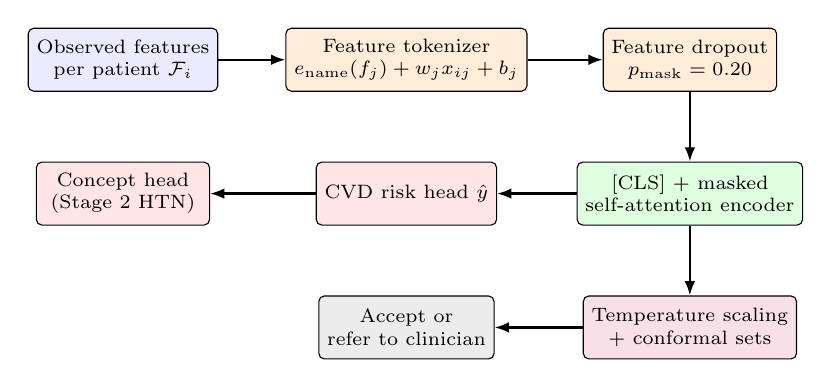
\begin{tikzpicture}[
  box/.style={draw,rounded corners=2pt,align=center,font=\scriptsize,minimum height=8mm,minimum width=22mm,inner sep=3pt},
  arr/.style={-{Latex[length=1.8mm]},thick}]
\node[box,fill=blue!8] (in) at (0,0) {Observed features\\ per patient $\mathcal{F}_i$};
\node[box,fill=orange!15] (tok) at (3.6,0) {Feature tokenizer\\$e_{\mathrm{name}}(f_j)+w_jx_{ij}+b_j$};
\node[box,fill=orange!15] (drop) at (7.2,0) {Feature dropout\\$p_{\mathrm{mask}}=0.20$};
\node[box,fill=green!12] (enc) at (7.2,-1.7) {[CLS] + masked\\ self-attention encoder};
\node[box,fill=red!10] (risk) at (3.6,-1.7) {CVD risk head $\hat y$};
\node[box,fill=red!10] (con) at (0,-1.7) {Concept head\\(Stage 2 HTN)};
\node[box,fill=purple!12] (cal) at (7.2,-3.4) {Temperature scaling\\+ conformal sets};
\node[box,fill=gray!15] (out) at (3.6,-3.4) {Accept or\\ refer to clinician};
\draw[arr] (in)--(tok); \draw[arr] (tok)--(drop); \draw[arr] (drop)--(enc);
\draw[arr] (enc)--(risk); \draw[arr] (risk)--(con); \draw[arr] (enc)--(cal);
\draw[arr] (cal)--(out);
\end{tikzpicture}}
\caption{\sfn{} pipeline. Only observed features are tokenized; absent features are masked in attention. A monotonicity penalty acts on $\partial\hat y/\partial x_k$ during training.}
\label{fig:arch}
\end{figure}

\subsection{Schema-flexible tokenizer}
For patient $i$ with observed feature set $\mathcal{F}_i$, each observed feature $j\in\mathcal{F}_i$ becomes a token
\begin{equation}
z_{ij}=e_{\mathrm{name}}(f_j)+w_j\,x_{ij}+b_j,
\end{equation}
where $e_{\mathrm{name}}(f_j)\in\mathbb{R}^d$ is a learned embedding that identifies the feature, and $(w_j,b_j)$ is a feature-specific linear projection (categorical variables use learned value embeddings). Continuous inputs are z-scored with training statistics. We prepend a learnable \texttt{[CLS]} token and use a key-padding mask to keep unobserved features out of attention, so there is no inner join, zero-fill or imputation. The encoder has 2 layers and 4 heads, width $d=64$, feed-forward width 128 and dropout 0.10.

\subsection{Feature dropout}
At training time every observed token is dropped with probability $p_{\mathrm{mask}}=0.20$. This mimics hospitals that report only part of the panel, and it stops the encoder from leaning on any one variable.

\subsection{Concept head and monotonicity}
The \texttt{[CLS]} representation also predicts Stage~2 hypertension, which adds the binary cross-entropy term $\mathcal{L}_{\mathrm{concept}}$. We push the model toward monotonicity in two ways, for the harmful markers $\mathcal{M}=\{$age, SBP, cholesterol, ST depression$\}$. The first is a residual branch in the logit whose weights pass through a softplus and are therefore non-negative:
\begin{equation}
\hat z_i=\mathbf{w}_{\mathrm{out}}^{\top}\mathbf{h}^{\mathrm{CLS}}_i+b_0+\sum_{k\in\mathcal{M}}\mathrm{softplus}(w_k)\,x_{ik}\,\mathbb{I}[x_{ik}\ \text{observed}],
\end{equation}
with $\hat y_i=\sigma(\hat z_i)$. Second, an input-gradient penalty computed by automatic differentiation,
\begin{equation}
\mathcal{L}_{\mathrm{mono}}=\frac{1}{|\mathcal{M}|}\sum_{k\in\mathcal{M}}\mathrm{ReLU}\!\left(-\frac{\partial \hat y_i}{\partial x_{i,k}}\right)\mathbb{I}[x_{i,k}\ \text{observed}].
\end{equation}
The total loss is
\begin{equation}
\mathcal{L}=\mathcal{L}_{\mathrm{BCE}}+\lambda_1\mathcal{L}_{\mathrm{concept}}+\lambda_2\mathcal{L}_{\mathrm{mono}},
\end{equation}
with $\lambda_1=0.10$ and $\lambda_2=1.20$. Nothing constrains the attention path, so neither mechanism guarantees monotonicity, and we \emph{measure} violations instead (Section~\ref{sec:ablation}).

\subsection{Calibration and conformal procedure}\label{sec:conformal_theory}
Split conformal prediction only gives valid distribution-free coverage when the data used to fit the model and the data used for conformal calibration are kept apart. If labeled calibration data are also used to fit a post-hoc probability calibration (temperature scaling, say) or to stop training early, optimization bias creeps in and the exchangeability argument no longer holds. We therefore use a \emph{three-way source partitioning protocol}:
\begin{enumerate}
\item \emph{Training split} ($D_{\mathrm{train}}$, 70\% of source pool): used only to fit the network parameters $\theta$.
\item \emph{Validation split} ($D_{\mathrm{val}}$, 15\% of source pool): used to pick the early-stopping checkpoint and to fit the scalar temperature $T^*$ with L-BFGS, by minimizing the negative log-likelihood of the uncalibrated logits $z(x)$.
\item \emph{Calibration split} ($D_{\mathrm{cal}}$, 15\% of source pool): a disjoint partition of $n$ patients that is never touched during training. Once $(\theta, T^*)$ are frozen, the calibrated probabilities $p_y(x) = \sigma(z(x)/T^*)$ give non-conformity scores $s(x,y) = 1 - p_y(x) \in [0, 1]$.
\end{enumerate}
Because $D_{\mathrm{cal}}$ is disjoint from both $D_{\mathrm{train}}$ and $D_{\mathrm{val}}$, the score function $s(x,y)$ is deterministic with respect to $D_{\mathrm{cal}}$. Given the fitted model, the scores on $D_{\mathrm{cal}}$ and on any i.i.d.\ test point $(X_{n+1}, Y_{n+1}) \sim P_{\mathrm{source}}$ are exchangeable.
At nominal error rate $\alpha=0.10$ ($1-\alpha=90\%$ target coverage), the finite-sample adjusted conformal quantile threshold is computed on $n$ calibration samples as:
\begin{equation}
\hat{q} = \mathrm{Quantile}\left(\{s(x_i, y_i)\}_{i=1}^n; \; \frac{\lceil (n+1)(1-\alpha) \rceil}{n}\right).
\end{equation}
The prediction set for a test patient $x$ is:
\begin{equation}
\begin{split}
\mathcal{C}(x) &= \{y \in \{0, 1\} : s(x, y) \le \hat{q}\}\\
&= \{y \in \{0, 1\} : p_y(x) \ge 1 - \hat{q}\}.
\end{split}
\end{equation}
Under source exchangeability, $\Pr[Y \in \mathcal{C}(X)] \ge 1 - \alpha$. We \emph{accept} a case when $|\mathcal{C}(x)|=1$ (a single label, with point prediction $\hat{y} = \arg\max_y p_y(x)$) and \emph{refer or abstain} when $|\mathcal{C}(x)| \in \{0, 2\}$. For Mondrian conformal calibration, $\hat{q}_g$ is computed separately for each biological sex $g \in \{\mathrm{Male}, \mathrm{Female}\}$.

\textbf{Mathematical upper bound on conformal coverage.} In binary classification on $N$ evaluation patients, every prediction set has size 0, 1 or 2, so $|\mathcal{C}(x_i)|\in\{0,1,2\}$. Write $N_0 = |\{i : |\mathcal{C}(x_i)|=0\}|$ for the number of empty sets, $N_1 = |\{i : |\mathcal{C}(x_i)|=1\}|$ for singleton sets (the accepted predictions, with $r_{\mathrm{acc}}=N_1/N$), and $N_2 = |\{i : |\mathcal{C}(x_i)|=2\}|$ for the uncertain pair sets ($\mathcal{C}(x_i)=\{0,1\}$), so $N=N_0+N_1+N_2$. The accepted patients have accuracy $\mathrm{Acc}_{\mathrm{acc}} = N_{1,\mathrm{corr}}/N_1$. When an accepted prediction is wrong, the set is $\mathcal{C}(x_i)=\{1-y_i\}$ and so does not contain the true label $y_i$. Empty sets contain no label either. The true label $y_i\in\mathcal{C}(x_i)$ is therefore covered only for correct singletons and for pair sets, giving $N_{\mathrm{cov}} = N_{1,\mathrm{corr}} + N_2 = (N_1 - N_{1,\mathrm{err}}) + (N - N_0 - N_1) = N - N_0 - N_{1,\mathrm{err}}$. Dividing by $N$ gives an exact identity for coverage:
\begin{equation}
\begin{split}
\mathrm{Coverage} &= \frac{N_{\mathrm{cov}}}{N} = 1 - \frac{N_0}{N} - r_{\mathrm{acc}}(1 - \mathrm{Acc}_{\mathrm{acc}})\\
&\le 1 - r_{\mathrm{acc}}(1 - \mathrm{Acc}_{\mathrm{acc}}),
\end{split}
\label{eq:conformal_bound}
\end{equation}
with equality exactly when there are no empty prediction sets ($N_0=0$). An empirical coverage above $1 - r_{\mathrm{acc}}(1 - \mathrm{Acc}_{\mathrm{acc}})$ would contradict this identity and so cannot be right. In leave-one-cohort-out use, calibrating on the source breaks exchangeability ($P_{\mathrm{source}}\neq P_{\mathrm{target}}$), and Section~\ref{sec:conformal} measures how far coverage drops as a result.

\subsection{Schema-aware federated averaging}
In the federated simulation each hospital node $h$ sees only a subset $\mathcal{F}_h$ of the features. The parameters shared across features (transformer blocks, \texttt{[CLS]}, heads) are averaged over all nodes, weighted by the local sample size $n_h$:
\begin{equation}
\theta_{\mathrm{shared}}\leftarrow\sum_h \frac{n_h}{\sum_{h'}n_{h'}}\,\theta^{(h)}_{\mathrm{shared}}.
\end{equation}
Feature-specific parameters $\theta_j=(e_{\mathrm{name}}(f_j),w_j,b_j)$ are averaged only over the nodes $H_j=\{h: j\in\mathcal{F}_h\}$ that observe feature $j$:
\begin{equation}
\theta_j\leftarrow\sum_{h\in H_j}\frac{n_h}{\sum_{h'\in H_j}n_{h'}}\,\theta^{(h)}_j.
\end{equation}
This way a feature's embeddings are not watered down by nodes that never observe it.

\subsection{Evaluation metrics}
Calibration is summarized by the expected calibration error over $B$ equal-width probability bins,
\begin{equation}
\mathrm{ECE}=\sum_{b=1}^{B}\frac{|S_b|}{N}\,\bigl|\mathrm{acc}(S_b)-\mathrm{conf}(S_b)\bigr|,
\end{equation}
and by the Brier score $\frac{1}{N}\sum_i(\hat y_i-y_i)^2$. Clinical utility at decision threshold $p_t$ is the net benefit
\begin{equation}
\mathrm{NB}(p_t)=\frac{TP}{N}-\frac{FP}{N}\cdot\frac{p_t}{1-p_t},
\end{equation}
compared with the treat-all strategy $\mathrm{NB}_{\mathrm{all}}=\pi-(1-\pi)\,p_t/(1-p_t)$, where $\pi$ is prevalence~\cite{vickers2006}.

%=====================================================================
\section{Experimental Protocol}\label{sec:protocol}
\textbf{Data partitioning and splits.} Each experimental track follows its own split protocol, fixed in advance.
\begin{enumerate}
\item \emph{Pooled multi-model benchmark ($N=74{,}013$):} stratified five-fold cross-validation on all non-overlapping records, with Statlog excluded. Each fold trains on 80\% ($N=59{,}210$) and tests on 20\% ($N=14{,}803$). Every model is run on raw features only and again with four engineered meta-features (\texttt{bmi}, \texttt{pulse\_pressure}, \texttt{chol\_tier}, \texttt{gluc\_tier}).
\item \emph{Literature 70/15/15 reproduction:} a stratified split into 70\% training, 15\% validation (used to select the early-stopping checkpoint) and 15\% held-out test. It is applied to the leaked pool (71{,}025 raw $\rightarrow$ 69{,}692 clean), the deduplicated pool (70{,}302 raw $\rightarrow$ 68{,}969 clean) and Sulianova alone (68{,}568 full QC / 68{,}667 minimal filter).
\item \emph{Leave-one-cohort-out (LOCO) cross-hospital transfer:} in each of five folds one whole cohort is held out as the unseen target ($N_{\mathrm{test}}$: Hungarian=293, VA+Switzerland=308, Cleveland=303, Z-Alizadeh Sani=303, Framingham=4{,}238). The other $K-1$ cohorts form the source pool ($N_{\mathrm{source}}\approx 69{,}775$--$73{,}720$), which is split strictly into 70\% training ($D_{\mathrm{train}}$, for fitting the network parameters $\theta$), 15\% validation ($D_{\mathrm{val}}$, for early stopping and the temperature $T^*$) and a disjoint 15\% calibration set ($D_{\mathrm{cal}}$, for calibrating the finite-sample non-conformity threshold $\hat{q}$). Zero-shot evaluation uses 100\% of the target records. For target recalibration, a stratified 20\% local slice ($D_{\mathrm{tgt,cal}}$) re-estimates the non-conformity quantiles and the remaining 80\% of the target is used for evaluation.
\item \emph{Missingness stress test and architectural ablation:} a stratified multi-cohort split into 70\% training, 15\% validation and 15\% held-out test ($N=11{,}102$ test patients, Statlog excluded).
\end{enumerate}

\textbf{Conformal calibration and decision rule.} With the temperature-scaled probability $p_y(x) = \hat{P}(Y=y \mid X=x)$, the non-conformity score is $s(x,y)=1-p_y(x)$. For nominal coverage $1-\alpha=0.90$ ($\alpha=0.10$), the quantile $\hat{q}$ is taken over $n$ calibration samples as $\hat{q} = \mathrm{Quantile}(\{s(x_i,y_i)\}_{i=1}^n; \; \lceil (n+1)(1-\alpha) \rceil / n)$, and the prediction set is $\mathcal{C}(x) = \{y \in \{0,1\} : s(x,y) \le \hat{q}\}$. A case is accepted if $|\mathcal{C}(x)|=1$ (a single label, with prediction $\hat{y}=\arg\max_y p_y(x)$) and referred or abstained if $|\mathcal{C}(x)|\in\{0,2\}$. Empirical set coverage obeys Eq.~(\ref{eq:conformal_bound}). Under Mondrian conformal prediction, $\hat{q}_g$ is computed separately for each biological sex $g\in\{\mathrm{Male},\mathrm{Female}\}$.

\textbf{Repeated seeds and variance reporting.}
\begin{itemize}
\item \emph{Missingness stress test (Table~\ref{tab:miss}):} to make sure random masking does not drive the result, we repeat everything over \textbf{five independent random seeds} ($[42, 100, 2026, 777, 999]$). All five model families (SchemaFlex, Unregularized Transformer, Native-NaN LightGBM, Native-NaN XGBoost, Median-Imputed LightGBM) get exactly the same masked subsets. We report the mean $\pm$ sample standard deviation.
\item \emph{LOCO cross-cohort matrix (Table~\ref{tab:loco}) and conformal abstention audit (Table~\ref{tab:conf}):} run over \textbf{five independent random seeds} ($[42, 100, 2026, 777, 999]$), with the mean $\pm$ sample standard deviation reported for every cohort. We add deterministic single-seed ($42$) patient-level count audits and paired DeLong tests with family-wise Holm--Bonferroni correction.
\item \emph{Subgroup analysis:} 95\% confidence intervals come from 1{,}000 bootstrap resamples.
\end{itemize}

\textbf{Model architecture and training optimization.} \sfn{} has 2 transformer layers, 4 attention heads, token embedding dimension $d=64$, feedforward dimension 128 and dropout $0.10$. We train with AdamW ($\beta_1=0.9, \beta_2=0.999$, weight decay $10^{-4}$), an initial learning rate of $1.5\times 10^{-3}$ annealed with a cosine schedule to $10^{-5}$ over 16 epochs, batch size 256 and gradient-norm clipping at $1.0$. The loss weights are fixed at $\lambda_{\mathrm{concept}}=0.10$ and $\lambda_{\mathrm{mono}}=1.20$. The tree baselines (LightGBM, XGBoost, CatBoost) are tuned with early stopping on validation AUROC. Prospective multi-site clinical validation is still needed.

%=====================================================================
\section{Results}\label{sec:results}
\subsection{Pooled benchmark}\label{sec:pooled}
In pooled stratified five-fold cross-validation (74{,}013 patients), LightGBM with raw plus engineered features reaches an AUROC of 0.8249 and 75.98\% accuracy (75.39\% on raw features alone). XGBoost, random forest and CatBoost stay within 0.004 AUROC of it, MLP and TabNet get about 0.811, and logistic regression 0.768 (Table~\ref{tab:pooled}). For the models we tried, these numbers look like a ceiling on this pool, and they sit well below 90\%. The engineered features help every model, by $+0.0014$ to $+0.0124$ AUROC.

\begin{table}[t]
\caption{Pooled 5-fold benchmark: AUROC with raw features (A) and with engineered meta-features (B); accuracy for B.}
\label{tab:pooled}
\centering\footnotesize
\begin{tabular}{lcccc}
\toprule
Model & A & B & $\Delta$ & Acc.\ B (\%)\\
\midrule
Logistic regression & 0.7554 & 0.7678 & $+0.0124$ & 70.19\\
Random forest & 0.8195 & 0.8244 & $+0.0049$ & 75.85\\
XGBoost & 0.8186 & 0.8247 & $+0.0061$ & 75.95\\
LightGBM & 0.8187 & 0.8249 & $+0.0062$ & 75.98\\
CatBoost & 0.8152 & 0.8215 & $+0.0063$ & 75.60\\
MLP & 0.8096 & 0.8110 & $+0.0014$ & 74.86\\
TabNet & 0.8078 & 0.8105 & $+0.0027$ & 74.87\\
\bottomrule
\end{tabular}
\end{table}

\subsection{Zero-shot cross-cohort transfer}
Table~\ref{tab:loco} and Fig.~\ref{fig:loco} give the LOCO transfer results over five repeated seeds ($[42, 100, 2026, 777, 999]$). The inner-join models do poorly (mean AUROC $0.6154 \pm 0.0054$ for LightGBM, 0.6445 for the re-implemented \htn{}) because the shared columns contain no chest-pain type, exercise ECG variables or vessel counts. What changes the picture is keeping the union schema: NaN-aware LightGBM then reaches $0.7405 \pm 0.0094$. \sfn{} gets $0.7635 \pm 0.0077$ (seed-42: 0.7662), a mean gain of $+0.0230$ over that stronger baseline. Most of it comes from Z-Alizadeh ($+0.0788$) and Hungarian ($+0.0199$). On VA+Switzerland \sfn{} is slightly lower ($-0.0032$), and on Cleveland ($+0.0092$) and Framingham ($+0.0103$) the two are about level.

Table~\ref{tab:delong} lists the paired DeLong tests. Compared with the re-implemented inner-join \htn{}, \sfn{} is significantly better on Hungarian ($p<10^{-10}$), VA+Switzerland ($p{=}5.6\times10^{-4}$) and Cleveland ($p{=}2.1\times10^{-6}$), and not significantly different on Z-Alizadeh ($p{=}0.84$) or Framingham ($p{=}0.71$). The comparison that tells us more is the one with union-schema LightGBM. Here the Z-Alizadeh gain is nominally significant (raw $p{=}0.037$), but once Holm correction is applied no cohort survives (adjusted $p\ge 0.18$). After correction we found no cohort-level AUROC difference between \sfn{} and union-schema LightGBM that reaches significance. Superiority is therefore not established by these tests, and the tests do not prove equivalence either. The tertiary cardiology cohorts have only about 300 patients ($N\approx 300$), so the power to detect small margins ($\Delta\approx 0.01$--$0.02$) is limited. To show practical equivalence one would need prespecified equivalence margins and a formal two one-sided test (TOST) on larger cohorts.

\begin{table*}[t]
\caption{Zero-shot LOCO AUROC across 5 repeated seeds (mean $\pm$ std; seed-42 point estimates in parentheses). Hybrid = re-implemented \htn{} with inner join; Union LGBM = NaN-aware LightGBM on the union schema. The mean row is the unweighted mean of the five per-cohort values. Bold marks the highest mean AUROC per row.}
\label{tab:loco}
\centering\footnotesize
\begin{tabular}{lccccc}
\toprule
Held-out cohort ($N$) & Inner-join LGBM & Hybrid (re-impl.) & Union LGBM & \sfn{} & $\Delta$ vs.\ union\\
\midrule
Hungarian (293) & 0.5979 $\pm$ 0.0060 (.605) & 0.6111 & 0.8433 $\pm$ 0.0128 (.856) & \textbf{0.8631 $\pm$ 0.0146} (.872) & $+0.0199$\\
VA+Switzerland (308) & 0.5419 $\pm$ 0.0041 (.538) & 0.5451 & \textbf{0.7262 $\pm$ 0.0091} (.729) & 0.7230 $\pm$ 0.0046 (.722) & $-0.0032$\\
Cleveland dedup.\ (303) & 0.5791 $\pm$ 0.0025 (.578) & 0.6785 & 0.8480 $\pm$ 0.0035 (.843) & \textbf{0.8572 $\pm$ 0.0085} (.855) & $+0.0092$\\
Z-Alizadeh Sani (303) & 0.6836 $\pm$ 0.0094 (.693) & \textbf{0.7126} & 0.6153 $\pm$ 0.0177 (.625) & 0.6942 $\pm$ 0.0085 (.701) & $+0.0788$\\
Framingham (4{,}238) & 0.6745 $\pm$ 0.0052 (.676) & 0.6750 & 0.6699 $\pm$ 0.0041 (.675) & \textbf{0.6802 $\pm$ 0.0024} (.681) & $+0.0103$\\
\midrule
Unweighted mean & 0.6154 $\pm$ 0.0054 (.618) & 0.6445 & 0.7405 $\pm$ 0.0094 (.745) & \textbf{0.7635 $\pm$ 0.0077} (.766) & $+0.0230$\\
\bottomrule
\end{tabular}
\end{table*}

\begin{table*}[t]
\caption{Paired DeLong tests for \sfn{} on seed-42 predictions. ``Union'' = union-schema NaN-aware LightGBM, with Holm--Bonferroni adjustment across the five cohorts. ``Hybrid'' = re-implemented inner-join \htn{} (unadjusted $p$). n.s.\ = not significant at 0.05.}
\label{tab:delong}
\centering\footnotesize
\begin{tabular}{lrcccccc}
\toprule
Held-out cohort & $N$ & $\Delta$ vs.\ union & DeLong $z$ & Raw $p$ & Holm $p$ & Sig.\ (Holm) & $p$ vs.\ Hybrid\\
\midrule
Hungarian & 293 & $+0.0218$ & 1.413 & 0.158 & 0.631 & n.s. & $<10^{-10}$\\
VA+Switzerland & 308 & $-0.0039$ & $-0.255$ & 0.798 & 1.000 & n.s. & $5.6\times10^{-4}$\\
Cleveland dedup. & 303 & $-0.0133$ & $-0.760$ & 0.447 & 1.000 & n.s. & $2.1\times10^{-6}$\\
Z-Alizadeh Sani & 303 & $+0.1015$ & 2.087 & 0.037 & 0.185 & n.s. & 0.84 (n.s.)\\
Framingham & 4{,}238 & $+0.0083$ & 0.722 & 0.470 & 1.000 & n.s. & 0.71 (n.s.)\\
\bottomrule
\end{tabular}
\end{table*}

\begin{figure}[t]
\centering
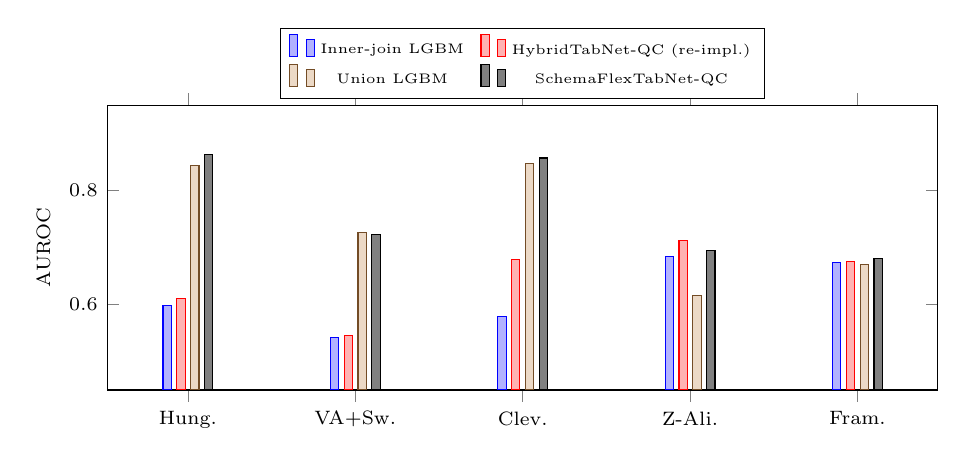
\begin{tikzpicture}
\begin{axis}[ybar,width=\columnwidth,height=5.2cm,bar width=3pt,
  symbolic x coords={Hung.,VA+Sw.,Clev.,Z-Ali.,Fram.},xtick=data,
  x tick label style={font=\scriptsize},y tick label style={font=\scriptsize},
  ylabel={AUROC},ylabel style={font=\scriptsize},ymin=0.45,ymax=0.95,
  legend style={font=\tiny,at={(0.5,1.02)},anchor=south,legend columns=2,/tikz/every even column/.append style={column sep=4pt}},
  enlarge x limits=0.12]
\addplot coordinates {(Hung.,0.5979) (VA+Sw.,0.5419) (Clev.,0.5791) (Z-Ali.,0.6836) (Fram.,0.6745)};
\addplot coordinates {(Hung.,0.6111) (VA+Sw.,0.5451) (Clev.,0.6785) (Z-Ali.,0.7126) (Fram.,0.6750)};
\addplot coordinates {(Hung.,0.8433) (VA+Sw.,0.7262) (Clev.,0.8480) (Z-Ali.,0.6153) (Fram.,0.6699)};
\addplot coordinates {(Hung.,0.8631) (VA+Sw.,0.7230) (Clev.,0.8572) (Z-Ali.,0.6942) (Fram.,0.6802)};
\legend{Inner-join LGBM,\htn{} (re-impl.),Union LGBM,\sfn{}}
\end{axis}
\end{tikzpicture}
\caption{Zero-shot AUROC by held-out cohort (5-seed mean values from Table~\ref{tab:loco}).}
\label{fig:loco}
\end{figure}

\subsection{Ablation and monotonicity}\label{sec:ablation}
Table~\ref{tab:abl} isolates each component on the held-out 15\% multi-cohort partition. One distinction matters. Variant 1 (inner join, AUROC 0.6342) works with only the 5 shared features, while Variant 2 (+ schema tokenizer, AUROC 0.8560) can use all 14 union features. To separate feature access from architecture, we trained a NaN-aware LightGBM on identical train, validation and test partitions with equivalent preprocessing, and it reached AUROC 0.8510 (vs.\ 0.6280 on the inner join). Most of the gain ($\approx$+0.223 AUROC) therefore comes from retaining the schema, that is, from keeping the specialized diagnostic variables. The schema-flexible tokenizer adds a further $+0.0050$ AUROC and the ability to take varying subsets of features without static imputation. A margin that small does not show that tabular transformers are generally better than gradient-boosted trees.
Feature dropout adds $+0.004$ AUROC and cuts monotonicity violations from 19.2\% to 4.2\%. The concept head changes AUROC by $+0.0007$ and raises violations to 13.0\%, so it is useful for interpretation rather than prediction. In Variant 5 the positive-constrained skip path and the autograd gradient penalty ($\lambda_2=1.20$) each regularize the input directional gradients. Together they lower the counterfactual monotonicity violation rate to 0.26\% on synthetic $+0.5$~SD perturbations of SBP and cholesterol, with no loss of discriminative power (0.8652 AUROC). Post-hoc temperature scaling works differently: it acts only on the output logits, reduces calibration error (ECE 0.0572) and leaves AUROC unchanged. The two serve different goals (physiological plausibility of the gradients vs.\ calibrated confidence) and should not be lumped together. These figures come from single runs without confidence intervals, and the evaluation split differs from that of Table~\ref{tab:loco}.

\begin{table}[t]
\caption{Component ablation on the held-out 15\% multi-cohort partition. Viol.\ = counterfactual monotonicity violations (\%).}
\label{tab:abl}
\centering\footnotesize
\begin{tabular}{p{2.9cm}rrrr}
\toprule
Variant & AUROC & Acc. & ECE & Viol.\\
\midrule
1. Inner-join, shared feats. & 0.6342 & 59.73 & 0.1368 & 15.04\\
2. + Schema tokenizer & 0.8560 & 75.77 & 0.1672 & 19.23\\
3. + Feature dropout & 0.8604 & 77.13 & 0.1008 & 4.18\\
4. + Concept head & 0.8611 & 77.82 & 0.1081 & 12.97\\
5. + Mono.\ + temperature & 0.8652 & 80.20 & 0.0572 & 0.26\\
\bottomrule
\end{tabular}
\end{table}

\subsection{Conformal abstention and cohort shift}\label{sec:conformal}
At $\alpha=0.10$ the model accepts between 46.5\% and 77.7\% of patients over 5 seeds, depending on the cohort (Table~\ref{tab:conf}). On the accepted cases AUROC goes up by 0.03--0.09 and accuracy by 5--12 points in the four tertiary cardiology cohorts. On Framingham accuracy hardly moves (51.3\% to 53.7\%), again because of outcome construct divergence. The accepted fraction is a \emph{selective-prediction rate} and not conformal coverage.

Table~\ref{tab:conf} gives the multi-seed LOCO conformal results (mean $\pm$ std over 5 seeds) next to a deterministic seed-42 patient-level count audit, which reconciles accepted accuracy and empirical set coverage with Eq.~(\ref{eq:conformal_bound}). Across all 25 runs (5 seeds $\times$ 5 cohorts) no empty prediction set occurred ($N_0=0$), so empirical set coverage coincides with the upper bound $1 - r_{\mathrm{acc}}(1 - \mathrm{Acc}_{\mathrm{acc}})$. Take the seed-42 audit on Hungarian ($N=293$): 213 singletons ($N_{1,\mathrm{corr}}=190$, $N_{1,\mathrm{err}}=23$, 89.2\% accuracy) and 80 pairs ($N_2=80, N_0=0$) give $N_{\mathrm{cov}}=270$, an empirical coverage of $270/293 = 92.15\%$, which equals $1 - (213/293)\times(1-0.8920) = 92.15\%$. On Cleveland ($N=303$), 212 singletons (177 correct, 35 errors) and 91 pairs give $N_{\mathrm{cov}}=268$ and coverage of $268/303 = 88.45\%$, the same as the ceiling of $88.45\%$. On Framingham ($N=4{,}238$) the accepted accuracy is 49.19\% over 2{,}968 singletons (1,460 correct, 1,508 errors); with 1{,}270 pairs and $N_0=0$ the empirical coverage is $2{,}730/4{,}238=64.42\%$, again equal to the bound of $64.42\%$. Averaged over 5 seeds, source coverage is 70.7\% on Framingham and 87.7--88.7\% on the tertiary cohorts (unweighted mean $84.6\% \pm 2.2\%$). A shift between cohorts therefore pulls marginal coverage below the nominal 90\%. Recalibrating on a 20\% local slice of the target brings coverage back to $89.7$--$95.1\%$ ($91.9\% \pm 2.6\%$ overall), since the non-conformity quantiles are then fitted to the target feature distribution.

\begin{table*}[t]
\caption{Multi-seed LOCO conformal abstention audit at $\alpha=0.10$ across 5 repeated seeds (mean $\pm$ std). Bracketed integer counts indicate the deterministic seed-42 patient audit ($N = N_1 + N_2 + N_0$, $N_0=0$). Max Bound = $1 - r_{\mathrm{acc}}(1 - \mathrm{Acc}_{\mathrm{acc}})$ from Eq.~(\ref{eq:conformal_bound}); Src.\ Cov.\ = $N_{\mathrm{cov}}/N$; Tgt.\ Cov.\ = coverage after 20\% target recalibration.}
\label{tab:conf}
\centering\footnotesize
\setlength{\tabcolsep}{3.5pt}
\resizebox{\ifdim\width>\textwidth\textwidth\else\width\fi}{!}{%
\begin{tabular}{lrcccccc}
\toprule
Held-out cohort & Test $N$ & Acceptance Rate $r_{\mathrm{acc}}$ [$N_1$] & Accepted Acc.\ (\%) & Src.\ Set Cov.\ & Max Bound & Tgt.\ Set Cov.\ & AUROC (All $\rightarrow$ Acc.)\\
\midrule
Hungarian & 293 & 77.7\% $\pm$ 4.5\% [213 (72.7\%)] & 85.5\% $\pm$ 2.2\% [89.2\%] & 88.7\% $\pm$ 2.0\% [92.2\%] & 88.7\% $\pm$ 2.0\% [92.2\%] & 91.2\% $\pm$ 4.3\% & .863 $\rightarrow$ .892 $\pm$ .014\\
VA+Switzerland & 308 & 65.6\% $\pm$ 2.9\% [200 (64.9\%)] & 81.3\% $\pm$ 2.7\% [78.5\%] & 87.8\% $\pm$ 1.4\% [86.0\%] & 87.8\% $\pm$ 1.4\% [86.0\%] & 92.6\% $\pm$ 1.8\% & .723 $\rightarrow$ .764 $\pm$ .018\\
Cleveland dedup. & 303 & 72.9\% $\pm$ 5.1\% [212 (70.0\%)] & 84.0\% $\pm$ 1.3\% [83.5\%] & 88.3\% $\pm$ 1.2\% [88.5\%] & 88.3\% $\pm$ 1.2\% [88.5\%] & 95.1\% $\pm$ 2.7\% & .857 $\rightarrow$ .898 $\pm$ .006\\
Z-Alizadeh Sani & 303 & 46.5\% $\pm$ 5.4\% [148 (48.8\%)] & 73.5\% $\pm$ 1.3\% [74.3\%] & 87.7\% $\pm$ 0.9\% [87.5\%] & 87.7\% $\pm$ 0.9\% [87.5\%] & 91.1\% $\pm$ 3.6\% & .694 $\rightarrow$ .719 $\pm$ .029\\
Framingham & 4{,}238 & 62.9\% $\pm$ 4.5\% [2968 (70.0\%)] & 53.7\% $\pm$ 5.9\% [49.2\%] & 70.7\% $\pm$ 5.3\% [64.4\%] & 70.7\% $\pm$ 5.3\% [64.4\%] & 89.7\% $\pm$ 0.4\% & .680 $\rightarrow$ .717 $\pm$ .010\\
\midrule
Unweighted Mean & --- & 65.1\% $\pm$ 4.5\% [65.3\%] & 75.6\% $\pm$ 2.7\% [74.9\%] & 84.6\% $\pm$ 2.2\% [83.7\%] & 84.6\% $\pm$ 2.2\% [83.7\%] & 91.9\% $\pm$ 2.6\% & .764 $\rightarrow$ .798 $\pm$ .015\\
\bottomrule
\end{tabular}}
\end{table*}

\subsection{Robustness to missing data}
Table~\ref{tab:miss} and Fig.~\ref{fig:miss} show AUROC when 0--50\% of the features are missing at test time, on the held-out 15\% multi-cohort partition. Every model sees the same feature dropout masks, and we average over 5 random seeds ($\pm$ standard deviation). Trained on the full 14-feature union schema, the tree baselines reach $\approx$0.811 AUROC with nothing missing (Native LightGBM 0.8107, Native XGBoost 0.8110, Median LightGBM 0.8105), in line with the pooled cross-validation band of Table~\ref{tab:pooled}. As features are removed, \sfn{} drops from 0.8520 to 0.7123 $\pm$ 0.0051 at 50\% missingness. It stays ahead of the split-routing native-NaN trees (+0.0279 over LightGBM, +0.0409 over XGBoost). Median-imputed LightGBM, however, keeps 0.7262 $\pm$ 0.0019 AUROC and beats both native-NaN trees and the unregularized transformer. This tempers the result. Token dropout gives a transformer a structural way to cope with unobserved inputs, but plain mean or median imputation in tree ensembles turns out to be very robust under random missingness. We therefore read the robustness comparison as provisional and dependent on the task, and not as a sign that neural models are better in general.

\begin{table}[t]
\caption{AUROC under test-time missing features across 5 repeated masking seeds (mean $\pm$ std). Native = native missing-value routing; Med.\ = median imputation; Unreg.\ = unregularized transformer.}
\label{tab:miss}
\centering\footnotesize
\setlength{\tabcolsep}{2.5pt}
\resizebox{\ifdim\width>\columnwidth\columnwidth\else\width\fi}{!}{%
\begin{tabular}{rccccc}
\toprule
Missing & \sfn{} & Unreg. & Native LGBM & Native XGB & Med.\ LGBM\\
\midrule
0\%  & .852 $\pm$ .000 & .838 $\pm$ .000 & .811 $\pm$ .000 & .811 $\pm$ .000 & .811 $\pm$ .000\\
10\% & .830 $\pm$ .002 & .802 $\pm$ .003 & .780 $\pm$ .003 & .782 $\pm$ .001 & .796 $\pm$ .002\\
20\% & .804 $\pm$ .003 & .777 $\pm$ .003 & .753 $\pm$ .004 & .756 $\pm$ .001 & .781 $\pm$ .003\\
30\% & .751 $\pm$ .004 & .729 $\pm$ .004 & .730 $\pm$ .004 & .730 $\pm$ .001 & .764 $\pm$ .003\\
40\% & .716 $\pm$ .005 & .696 $\pm$ .005 & .708 $\pm$ .005 & .700 $\pm$ .002 & .746 $\pm$ .003\\
50\% & .712 $\pm$ .005 & .699 $\pm$ .005 & .684 $\pm$ .007 & .671 $\pm$ .004 & .726 $\pm$ .002\\
\bottomrule
\end{tabular}}
\end{table}

\begin{figure}[t]
\centering
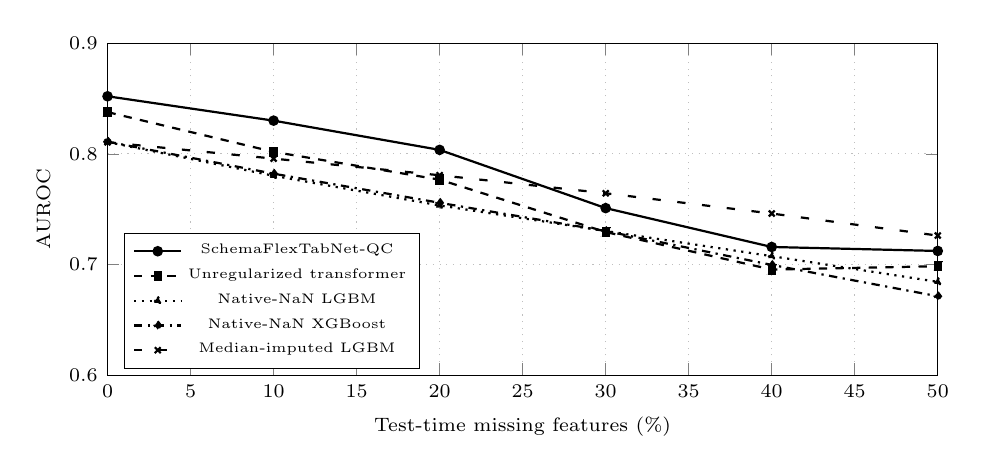
\begin{tikzpicture}
\begin{axis}[width=\columnwidth,height=5.8cm,xlabel={Test-time missing features (\%)},ylabel={AUROC},
  xlabel style={font=\scriptsize},ylabel style={font=\scriptsize},
  tick label style={font=\scriptsize},legend style={font=\tiny,at={(0.02,0.02)},anchor=south west},
  xmin=0,xmax=50,ymin=0.6,ymax=0.9,grid=major,grid style={dotted}]
\addplot[thick,mark=*,mark size=1.5pt] coordinates {(0,0.8520)(10,0.8300)(20,0.8036)(30,0.7510)(40,0.7159)(50,0.7123)};
\addplot[thick,dashed,mark=square*,mark size=1.5pt] coordinates {(0,0.8377)(10,0.8018)(20,0.7767)(30,0.7294)(40,0.6955)(50,0.6985)};
\addplot[thick,dotted,mark=triangle*,mark size=1.5pt] coordinates {(0,0.8107)(10,0.7802)(20,0.7534)(30,0.7303)(40,0.7076)(50,0.6844)};
\addplot[thick,dashdotted,mark=diamond*,mark size=1.5pt] coordinates {(0,0.8110)(10,0.7821)(20,0.7558)(30,0.7303)(40,0.6997)(50,0.6714)};
\addplot[thick,loosely dashed,mark=x,mark size=1.5pt] coordinates {(0,0.8105)(10,0.7957)(20,0.7807)(30,0.7644)(40,0.7461)(50,0.7262)};
\legend{\sfn{},Unregularized transformer,Native-NaN LGBM,Native-NaN XGBoost,Median-imputed LGBM}
\end{axis}
\end{tikzpicture}
\caption{Structured-missingness stress test across 5 repeated seeds (data of Table~\ref{tab:miss}).}
\label{fig:miss}
\end{figure}

\subsection{Fairness, federation and clinical utility}
\textbf{Subgroups.} In the 270-patient overlap cohort the false-positive rates are 0.398 for men and 0.119 for women, with sensitivities of 0.86 and 0.80; the age $>65$ group has only 30 patients. In a separate 298-patient evaluation, marginal conformal calibration gave FPRs of 0.038 (male) and 0.186 (female), and Mondrian calibration changed them to 0.173 and 0.246. It \emph{halved} the gap in FPR between the sexes, from 0.149 to 0.072 (a 51\% reduction), and lowered the male FNR from 0.395 to 0.250. The gap did not disappear, however, and the FPR rose in both groups. These subgroups are too small for the confidence intervals to support firm conclusions.

\textbf{Federated simulation.} We simulated four nodes. Schema-aware averaging, where feature-specific parameters are averaged only across the nodes that observe the feature, reaches 0.767 AUROC after 10 rounds, against 0.746 for isolated models and 0.875 for centralized training. Federation closes 16.3\% of the gap between isolated and centralized training. Only model weights are shared, and no formal privacy mechanism (differential privacy, secure aggregation) was used, so ``no row sharing'' should not be taken as a privacy guarantee.

\textbf{Decision curves.} On the same 270-patient cohort (prevalence 44.4\%), net benefit is above treat-all for thresholds from 0.10 to 0.30, for example 0.346 vs.\ 0.306 at 0.20, which corresponds to about four extra net true-positive decisions per 100 patients. This is one high-prevalence, single-center cohort, so the result should not be generalized.

%=====================================================================
\section{Discussion and Limitations}\label{sec:discussion}
\textbf{What the evidence supports.} Duplicates and cross-cohort record overlap are real and common in popular files, and they make random-split benchmarks unreliable. Inner-join harmonization badly hurts cross-cohort transfer because the clinical measurements that are not shared get thrown away. Keeping the union schema recovers most of that loss, whether with masked transformers or with NaN-aware trees. The transformer adds a modest mean gain ($+0.023$ AUROC) that is not statistically significant for any single cohort after Holm correction. It also copes structurally with missing inputs at test time and allows conformal abstention, but it is not uniformly better.

\textbf{What it does not support.} We have not shown that duplicate contamination explains the 90.1\% published in~\cite{mahmud2026}. The fixed-prediction bound and the controlled retraining both say that duplicates move accuracy by only $\sim$0.30 percentage points, so where that figure comes from is still unknown. We do not claim to have refuted, architecture for architecture, the proprietary transformer in~\cite{mahmud2026}, and we do not claim equivalence to union-schema LightGBM.

\subsection{Outcome-construct divergence}
A central validity problem in multi-cohort cardiovascular benchmarks is that the outcome means different things in different cohorts. The merged binary label combines three targets that differ clinically and in time:
\begin{enumerate}
\item \emph{Prevalent cardiovascular disease at examination} (Sulianova CVD, $N{=}68{,}568$): cross-sectional clinical history and screening findings.
\item \emph{Angiographic coronary artery disease} (UCI cohorts, Z-Alizadeh Sani, $N{=}1{,}207$): acute objective visualization of $\ge 50\%$ luminal stenosis on cardiac catheterization.
\item \emph{Incident coronary heart disease events during longitudinal follow-up} (Framingham Study, $N{=}4{,}238$): 10-year prospective event occurrence~\cite{dawber1951}.
\end{enumerate}
All three are stored as a binary label, but they are different prediction problems: detecting acute anatomical stenosis on one side, and prognosis over 10 years of prospective follow-up on the other. This divergence explains why transfer to Framingham stays flat (AUROC $\approx 0.670$--$0.680$ for all models) and why conformal set coverage collapses to 70.7\% $\pm$ 5.3\% (seed-42: 64.4\%), with singleton accuracy of only 53.7\% $\pm$ 5.9\% (seed-42: 49.2\%). Benchmarks that merge cohorts should not pool unlike clinical targets, or else should use prediction heads specific to each construct.

\textbf{Limitations.}
\begin{enumerate}
\item \emph{Outcome construct heterogeneity}, as discussed above. Mixing cross-sectional examination findings with 10-year incident events limits what the pooled predictions can mean clinically.
\item \emph{Pool composition imbalance.} Sulianova supplies 92.6\% of the records, so what the model learns about the specialized cardiology variables rests on a small minority of patients.
\item \emph{Conformal validity under cohort shift.} Calibrated on the source, coverage is 70.7\% on Framingham and 87.7--88.7\% on the tertiary cohorts (84.6\% $\pm$ 2.2\% unweighted mean; seed-42: 64.4--92.2\%), against a nominal 90\%. Eq.~(\ref{eq:conformal_bound}) bounds it by the accepted accuracy, and without local adaptation the conformal guarantee does not hold under distribution shift.
\item \emph{Statistical power and equivalence testing.} With about 300 patients per cohort ($N\approx 300$), small AUROC differences are hard to detect, and failing to reach significance after Holm correction is no evidence of practical equivalence.
\item \emph{Comparative tree robustness is provisional and context-dependent.} \sfn{} beats native-NaN split-routing trees at 50\% missingness (0.712 vs.\ 0.684), but median-imputed LightGBM reaches 0.726. Trees with simple imputation thus stay competitive when data are missing, and neural models have no general edge here.
\item \emph{Ablation interpretation.} Retaining the schema accounts for most of the gain ($\approx$+0.223 AUROC) and the tokenizer architecture for a further $+0.0050$ AUROC. Monotonicity regularization and post-hoc temperature scaling also pursue different clinical goals (gradient plausibility vs.\ probability calibration) and should be kept apart.
\item \emph{Reproduction scope.} Our 70/15/15 reproduction shows that standard tabular models reach $\approx$73\% on the published features. It is not a faithful reproduction of the unreleased neural code.
\item \emph{Patient identity verification.} Matching on feature signatures shows that records overlap at the row level. Without hospital records it cannot show that two rows belong to the same person.
\item \emph{No prospective clinical validation.} The model is a prototype for investigating benchmarks and is not an approved diagnostic tool.
\end{enumerate}

%=====================================================================
\section{Recommended Practice for Cardiovascular Benchmarks}\label{sec:practice}
Our audit points to a short checklist that would have avoided the problems described above and is cheap to adopt.
\begin{enumerate}
\item \emph{Deduplicate before splitting}. Use exact and near-duplicate signature matching on clinical features, and report how many rows were removed from each source.
\item \emph{Split at the patient level}. Where several files come from one registry, check for overlap between them before running any cross-cohort evaluation.
\item \emph{Report the pooled composition}, meaning each source's share of the records and the outcome definition it uses.
\item \emph{Compare against the strongest tree baseline}, with native missing-value handling and the same engineered features as the proposed model.
\item \emph{Evaluate on a held-out cohort} and not only on a random split of the pool, and report intervals and seed variance.
\item \emph{Report conformal set coverage and acceptance rate separately}, and check coverage on a different cohort before calling a system safe.
\item \emph{Reconcile every reported number}, so that text, tables and figures (confusion matrices, for example) imply the same metrics.
\item \emph{Publish code, splits and an audit log}, as TRIPOD+AI~\cite{collins2024} recommends.
\end{enumerate}
Items 1--2 alone would already remove the most extreme inflation we saw in public heart-disease files (Table~\ref{tab:leak}).

%=====================================================================
\section{Conclusion}\label{sec:conclusion}
Headline accuracies on public cardiovascular benchmarks deserve suspicion until the duplicates, cross-cohort overlap and schema loss have been checked. Once the data are cleaned, realistic accuracy on pooled routine data is about 73--76\%. Reproducing a published 90.1\% setup (70/15/15) with standard tabular baselines gives about 73\% with or without the duplicates, although that does not refute unreleased proprietary neural code. How well a model transfers between hospitals depends mostly on whether the unshared variables are kept, and much less on architectural novelty. \sfn{} offers a principled way of training across non-identical schemas. It gains a little on average over a strong NaN-aware tree baseline, but no cohort-level gain is significant after Holm correction. With 50\% of features missing at test time it beats native-NaN LightGBM and XGBoost by about 0.028 and 0.041 AUROC, respectively, yet median-imputed LightGBM (0.726) does better than it, so general superiority under missingness is not established. Its conformal coverage guarantee also weakens under cohort shift. These claims need multi-seed evaluation and prospective validation to be firmed up. We release the audit log, schema registry and code so that others can verify the work independently.

\section*{Data and Code Availability}
All datasets are public. Open-source code, configuration files, clean dataset splits and reproducible artifact CSVs are archived on GitHub: \url{https://github.com/RathanPaida/SchemaFlexTabNet-QC}. Table~\ref{tab:manifest} gives the complete end-to-end reproducibility manifest, mapping every empirical table in this manuscript to its script, configuration file, data partitioning protocol and artifact file in \texttt{results/}.

\begin{table*}[t]
\caption{End-to-End Reproducibility Manifest. Every empirical table in this manuscript is deterministically linked to an automated pipeline script, configuration file, data split protocol, and verified artifact file in \texttt{results/}.}
\label{tab:manifest}
\centering\footnotesize
\setlength{\tabcolsep}{3.8pt}
\resizebox{\ifdim\width>\textwidth\textwidth\else\width\fi}{!}{%
\begin{tabular}{lllll}
\toprule
Manuscript Item & Generating Pipeline Script & Primary Config & Data Split Protocol & Output CSV / Artifact File\\
\midrule
Table~\ref{tab:schema} (Feature Registry) & \texttt{src/data\_harmonizer.py} & \texttt{configs/schema\_registry.yaml} & Canonical definition ($M{=}14, C{=}1$) & \texttt{configs/schema\_registry.yaml}\\
Table~\ref{tab:cohorts} (Cohort Summary) & \texttt{src/data\_harmonizer.py} & \texttt{configs/schema\_registry.yaml} & 6 source cohorts ($N=74{,}013$) & \texttt{data/processed/clean\_multi\_cohort.parquet}\\
Table~\ref{tab:audit} (QC Audit Log) & \texttt{src/data\_harmonizer.py} & \texttt{configs/schema\_registry.yaml} & Physiological bounds gatekeeper & \texttt{results/table1\_forensic\_audit.csv}\\
Table~\ref{tab:leak} (Duplicate Leakage) & \texttt{src/reproducibility\_mahmud.py} & Default trees & Random 80/20 vs.\ deduplicated & \texttt{results/table1\_forensic\_audit.csv}\\
Table~\ref{tab:repro} (70/15/15 Repro.) & \texttt{src/reproducibility\_mahmud.py} & Default trees / MLP & 70/15/15 on raw, dedup, Sulianova & \texttt{results/mahmud\_reproduction\_audit.csv}\\
Table~\ref{tab:pooled} (Pooled 5-Fold) & \texttt{src/baseline\_models.py} & Default models & Stratified 5-fold CV ($N=74{,}013$) & \texttt{results/table2\_baseline\_benchmarking.csv}\\
Table~\ref{tab:loco} (5-Seed LOCO AUROC) & \texttt{evaluate\_multiseed\_loco\_and\_conformal.py} & \texttt{configs/schema\_registry.yaml} & LOCO 5 folds $\times$ 5 seeds (70/15/15) & \texttt{results/table4\_multiseed\_loco\_summary.csv}\\
Table~\ref{tab:delong} (Paired DeLong) & \texttt{src/statistical\_tests.py} & Holm--Bonferroni & LOCO fold predictions vs.\ Union & \texttt{results/table3\_proposed\_loco\_conformal.csv}\\
Table~\ref{tab:abl} (Ablation \& Mono.) & \texttt{src/ablation\_study.py} & \texttt{configs/schema\_registry.yaml} & 70/15/15 multi-cohort ($N=11{,}102$) & \texttt{results/table5\_ablation\_monotonicity.csv}\\
Table~\ref{tab:conf} (Conformal Audit) & \texttt{evaluate\_multiseed\_loco\_and\_conformal.py} & $\alpha=0.10$, 3-way split & LOCO 5 folds $\times$ 5 seeds & \texttt{results/loco\_multi\_seed\_stability\_audit.csv}\\
Table~\ref{tab:miss} (5-Seed Missingness) & \texttt{src/missingness\_experiment.py} & 5 masking seeds & 0--50\% test-time feature dropout & \texttt{results/table6\_missingness\_native\_nan.csv}\\
\bottomrule
\end{tabular}}
\end{table*}

%=====================================================================
\begin{thebibliography}{99}
\bibitem{mahmud2026} F. Mahmud \emph{et al.}, ``HybridTabNet-QC: A transformer-based clinical feature fusion framework for heart disease risk prediction,'' \emph{IEEE Open J. Comput. Soc.}, vol.~7, 2026, doi: 10.1109/OJCS.2025.3637308.
\bibitem{dua2019} D. Dua and C. Graff, ``UCI Machine Learning Repository,'' Univ.\ California, Irvine, 2019.
\bibitem{detrano1989} R. Detrano \emph{et al.}, ``International application of a new probability algorithm for the diagnosis of coronary artery disease,'' \emph{Am. J. Cardiol.}, vol.~64, no.~5, pp.~304--310, 1989.
\bibitem{alizadehsani2013} R. Alizadehsani \emph{et al.}, ``A data mining approach for diagnosis of coronary artery disease,'' \emph{Comput. Methods Programs Biomed.}, vol.~111, no.~1, pp.~52--61, 2013.
\bibitem{dawber1951} T. R. Dawber, G. F. Meadors, and F. E. Moore, ``Epidemiological approaches to heart disease: The Framingham Study,'' \emph{Am. J. Public Health}, vol.~41, no.~3, pp.~279--281, 1951.
\bibitem{kapoor2023} S. Kapoor and A. Narayanan, ``Leakage and the reproducibility crisis in machine-learning-based science,'' \emph{Patterns}, vol.~4, no.~9, p.~100804, 2023.
\bibitem{barz2020} B. Barz and J. Denzler, ``Do we train on test data? Purging CIFAR of near-duplicates,'' \emph{J. Imaging}, vol.~6, no.~6, p.~41, 2020.
\bibitem{gorishniy2021} Y. Gorishniy, I. Rubachev, V. Khrulkov, and A. Babenko, ``Revisiting deep learning models for tabular data,'' in \emph{Proc. NeurIPS}, vol.~34, 2021, pp.~18932--18943.
\bibitem{arik2021} S. {\"O}. Arik and T. Pfister, ``TabNet: Attentive interpretable tabular learning,'' in \emph{Proc. AAAI}, vol.~35, no.~8, 2021, pp.~6679--6687.
\bibitem{somepalli2021} G. Somepalli \emph{et al.}, ``SAINT: Improved neural networks for tabular data via row attention and contrastive pre-training,'' arXiv:2106.01342, 2021.
\bibitem{ke2017} G. Ke \emph{et al.}, ``LightGBM: A highly efficient gradient boosting decision tree,'' in \emph{Proc. NeurIPS}, vol.~30, 2017.
\bibitem{koh2020} P. W. Koh \emph{et al.}, ``Concept bottleneck models,'' in \emph{Proc. ICML}, 2020, pp.~5338--5348.
\bibitem{gupta2016} M. Gupta \emph{et al.}, ``Monotonic calibrated interpolated look-up tables,'' \emph{J. Mach. Learn. Res.}, vol.~17, no.~109, pp.~1--47, 2016.
\bibitem{guo2017} C. Guo, G. Pleiss, Y. Sun, and K. Q. Weinberger, ``On calibration of modern neural networks,'' in \emph{Proc. ICML}, 2017, pp.~1321--1330.
\bibitem{vovk2005} V. Vovk, A. Gammerman, and G. Shafer, \emph{Algorithmic Learning in a Random World}. Springer, 2005.
\bibitem{angelopoulos2023} A. N. Angelopoulos and S. Bates, ``Conformal prediction: A gentle introduction,'' \emph{Found. Trends Mach. Learn.}, vol.~16, no.~4, pp.~494--591, 2023.
\bibitem{tibshirani2019} R. J. Tibshirani, R. F. Barber, E. J. Cand{\`e}s, and A. Ramdas, ``Conformal prediction under covariate shift,'' in \emph{Proc. NeurIPS}, vol.~32, 2019.
\bibitem{barber2023} R. F. Barber, E. J. Cand{\`e}s, A. Ramdas, and R. J. Tibshirani, ``Conformal prediction beyond exchangeability,'' \emph{Ann. Statist.}, vol.~51, no.~2, pp.~816--845, 2023.
\bibitem{delong1988} E. R. DeLong, D. M. DeLong, and D. L. Clarke-Pearson, ``Comparing the areas under two or more correlated receiver operating characteristic curves: A nonparametric approach,'' \emph{Biometrics}, vol.~44, no.~3, pp.~837--845, 1988.
\bibitem{vickers2006} A. J. Vickers and E. B. Elkin, ``Decision curve analysis: A novel method for evaluating prediction models,'' \emph{Med. Decis. Making}, vol.~26, no.~6, pp.~565--574, 2006.
\bibitem{mcmahan2017} B. McMahan \emph{et al.}, ``Communication-efficient learning of deep networks from decentralized data,'' in \emph{Proc. AISTATS}, 2017, pp.~1273--1282.
\bibitem{collins2024} G. S. Collins \emph{et al.}, ``TRIPOD+AI statement: Updated guidance for reporting clinical prediction models that use regression or machine learning methods,'' \emph{BMJ}, vol.~385, p.~e078378, 2024.
\end{thebibliography}

\end{document}
